% This is samplepaper.tex, a sample chapter demonstrating the
% LLNCS macro package for Springer Computer Science proceedings;
% Version 2.20 of 2017/10/04
%
\documentclass[runningheads]{llncs}
%
\usepackage{times}
\usepackage{soul}
\usepackage{url}
\usepackage[hidelinks]{hyperref}
\usepackage[utf8]{inputenc}
%\usepackage[small]{caption}
\usepackage{graphicx}
\usepackage{amsmath}
%\usepackage{amsthm}
\usepackage{booktabs}
%\usepackage{algorithm}
%\usepackage{algorithmic}

\usepackage{enumerate}
\usepackage[linesnumbered,boxed]{algorithm2e}
\usepackage{amstext}
\usepackage{amssymb}
\usepackage{color}
\urlstyle{same}



\usepackage{caption}
\usepackage{subfig}
%\usepackage{subfigure}

% Used for displaying a sample figure. If possible, figure files should
% be included in EPS format.
%
% If you use the hyperref package, please uncomment the following line
% to display URLs in blue roman font according to Springer's eBook style:
% \renewcommand\UrlFont{\color{blue}\rmfamily}

\begin{document}
%
%\title{Forgeting in $\mu$-calculus\thanks{Supported by organization x.}}
\title{On the Weakest Sufficient Conditions in Propositional $\mu$-calculus}
% %
% %\titlerunning{Abbreviated paper title}
% % If the paper title is too long for the running head, you can set
% % an abbreviated paper title here
% %
% \author{First Author\inst{1}\orcidID{0000-1111-2222-3333} \and
% Second Author\inst{2,3}\orcidID{1111-2222-3333-4444} \and
% Third Author\inst{3}\orcidID{2222--3333-4444-5555}}
% %
% \authorrunning{F. Author et al.}
% % First names are abbreviated in the running head.
% % If there are more than two authors, 'et al.' is used.
% %
% \institute{Princeton University, Princeton NJ 08544, USA \and
% Springer Heidelberg, Tiergartenstr. 17, 69121 Heidelberg, Germany
% \email{lncs@springer.com}\\
% \url{http://www.springer.com/gp/computer-science/lncs} \and
% ABC Institute, Rupert-Karls-University Heidelberg, Heidelberg, Germany\\
% \email{\{abc,lncs\}@uni-heidelberg.de}}
% %

\newcommand{\tuple}[1]{{\langle{#1}\rangle}}
%\newcommand{\Dtuple}[2]{{\right\|{#2}\right\|}}
\newcommand{\Mod}{\textit{Mod}}
\newcommand\ie{{\it i.e. }}
\newcommand\eg{{\it e.g.}}
% \newcommand\st{{\it s.t. }}
% \newtheorem{definition}{Definition}
\newtheorem{examp}{Example}
% \newenvironment{example}{\begin{examp}\rm}{\end{examp}}
% \newtheorem{lemma}{Lemma}
% \newtheorem{proposition}{Proposition}
% \newtheorem{theorem}{Theorem}
% \newtheorem{corollary}[theorem]{Corollary}
\iffalse
\newenvironment{proof}{{\bf Proof:}}{\hfill\rule{2mm}{2mm}\\ }
\fi
\newcommand{\rto}{\rightarrow}
\newcommand{\lto}{\leftarrow}
\newcommand{\lrto}{\leftrightarrow}
\newcommand{\Rto}{\Rightarrow}
\newcommand{\Lto}{\Leftarrow}
\newcommand{\LRto}{\Leftrightarrow}
\newcommand{\Var}{\textit{Var}}
\newcommand{\Forget}{\textit{Forget}}
\newcommand{\KForget}{\textit{KForget}}
\newcommand{\TForget}{\textit{TForget}}
\newcommand{\forget}{\textit{forget}}
\newcommand{\Fst}{\textit{Fst}}
\newcommand{\dep}{\textit{dep}}
\newcommand{\term}{\textit{term}}
\newcommand{\literal}{\textit{literal}}

\newcommand{\Atom}{\mathcal{A}}
\newcommand{\SFive}{\textbf{S5}}
\newcommand{\MPK}{\textsc{k}}
\newcommand{\MPB}{\textsc{b}}
\newcommand{\MPT}{\textsc{t}}
\newcommand{\MPA}{\forall}
\newcommand{\MPE}{\exists}

\newcommand{\DNF}{\textit{DNF}}
\newcommand{\CNF}{\textit{CNF}}

\newcommand{\degree}{\textit{degree}}
\newcommand{\sunfold}{\textit{sunfold}}

\newcommand{\Pos}{\textit{Pos}}
\newcommand{\Neg}{\textit{Neg}}
\newcommand\wrt{{\it w.r.t.}}
\newcommand{\Hm} {{\cal M}}
\newcommand{\Hw} {{\cal W}}
\newcommand{\Hr} {{\cal R}}
\newcommand{\Hb} {{\cal B}}
\newcommand{\Ha} {{\cal A}}

\newcommand{\Dsj}{\triangledown}

\newcommand{\wnext}{\widetilde{\bigcirc}}
\newcommand{\nex}{\bigcirc}
\newcommand{\ness}{\square}
\newcommand{\qness}{\boxminus}
\newcommand{\wqnext}{\widetilde{\circleddash}}
\newcommand{\qnext}{\circleddash}
\newcommand{\may}{\lozenge}
\newcommand{\qmay}{\blacklozenge}
\newcommand{\unt} {{\cal U}}
\newcommand{\since} {{\cal S}}
\newcommand{\SNF} {\textit{SNF$_C$}}
\newcommand{\start}{\textbf{start}}
\newcommand{\Elm}{\textit{Elm}}
\newcommand{\simp}{\textbf{simp}}
\newcommand{\nnf}{\textbf{nnf}}

\newcommand{\Diff}{\textrm{Diff}}

\newcommand{\CTL}{\textrm{CTL}}
\newcommand{\Ind}{\textrm{Ind}}
\newcommand{\Tran}{\textrm{Tran}}
\newcommand{\Sub}{\textrm{Sub}}
\newcommand{\NI}{\textrm{NI}}
\newcommand{\Inst}{\textrm{Inst}}
\newcommand{\Com}{\textrm{Com}}
\newcommand{\Rp}{\textrm{Rp}}
%\newcommand{\forget}{{\textsc{f}_\CTL}}
\newcommand{\ALL}{\textsc{a}}
\newcommand{\EXIST}{\textsc{e}}
\newcommand{\NEXT}{\textsc{x}}
\newcommand{\FUTURE}{\textsc{f}}
\newcommand{\UNTIL}{\textsc{u}}
\newcommand{\GLOBAL}{\textsc{g}}
\newcommand{\UNLESS}{\textsc{w}}
\newcommand{\Def}{\textrm{def}}
\newcommand{\IR}{\textrm{IR}}
\newcommand{\Tr}{\textrm{Tr}}
\newcommand{\dis}{\textrm{dis}}
\def\PP{\ensuremath{\textbf{PP}}}
\def\NgP{\ensuremath{\textbf{NP}}}
\def\W{\ensuremath{\textbf{W}}}
\newcommand{\Pre}{\textrm{Pre}}
\newcommand{\Post}{\textrm{Post}}


\newcommand{\CTLsnf}{{\textsc{SNF}_{\textsc{ctl}}^g}}
\newcommand{\ResC}{{\textsc{R}_{\textsc{ctl}}^{\succ, S}}}
\newcommand{\CTLforget}{{\textsc{F}_{\textsc{ctl}}}}
\newcommand{\Muforget}{{\textsc{F}_{\textsc{$\mu$}}}}
\newcommand{\Refine}{\textsc{Refine}}
\newcommand{\cf}{\textrm{cf.}}
\newcommand{\NEXP}{\textmd{\rm NEXP}}
\newcommand{\EXP}{\textmd{\rm EXP}}
\newcommand{\coNEXP}{\textmd{\rm co-NEXP}}
\newcommand{\NP}{\textmd{\rm NP}}
\newcommand{\coNP}{\textmd{\rm co-NP}}
\newcommand{\Pol}{\textmd{\rm P}}
\newcommand{\BH}[1]{\textmd{\rm BH}_{#1}}
\newcommand{\coBH}[1]{\textmd{\rm co-BH}_{#1}}
\newcommand{\Empty}{\emptyset}%\varnothing}
\newcommand{\NLOG}{\textmd{\rm NLOG}}
\newcommand{\DeltaP}[1]{\Delta_{#1}^{p}}
\newcommand{\PIP}[1]{\Pi_{#1}^{p}}
\newcommand{\SigmaP}[1]{\Sigma_{#1}^{p}}


\maketitle              % typeset the header of the contribution
%
\begin{abstract}
The $\mu$-calculus is one of the most important logics describing specifications of transition systems. It has been
extensively explored for formal verification in model checking due to its exceptional balance between expressiveness and algorithmic properties.
On the one hand, some  information content in a specification
might become irrelevant or unnecessary due to various reasons from the perspective of knowledge representation.
On the other hand, a weakest precondition of a specification is badly necessary in verification, where
 a (weakest) precondition is sufficient for a transition system to enjoy a desire property.
 This paper is to address these scenarios for $\mu$-calculus in a principle way in terms of knowledge {\em forgetting}.
In particular, it proposes a
notion of forgetting by a generalized bisimilar equivalence (over a signature) and explores
its important properties as a knowledge distilling operator, besides some reasoning complexity results.
It then shows that how the weakest sufficient condition and the strongest necessary condition can be established
via forgetting. It also discusses knowledge update for $\mu$-calculus in terms of forgetting.

% Propositional $\mu$-calculus is an expressive logic, and also an important specification language in verification.
% One of the common phenomenons in both the verification and the system design is some information content of such specification might become irrelevant for the system due to various reasons e.g., it might be discarded or become obsolete by time, or just become infeasible due to practical difficulties.
% Then, the problem arises on how to distill the information without altering the relevant system behavior or violating the original specification over a given signature.
% Moreover, three crucial notions are vital:  the \emph{strongest necessary condition} (SNC), the \emph{weakest sufficient condition}  (WSC) and the knowledge update.
% To address these scenarios and to target the relevant notions SNC (WSC) and knowledge update in a principled way. In this paper, we explore the knowledge update and SNC (WSC) of $\mu$-calculus from the point of \emph{forgetting}.
% We study its theoretical properties and also show that our notion
% of forgetting satisfies existing essential postulates of knowledge forgetting.
% Furthermore, we show that the reasoning problems of the forgetting are $\textsc{Exptime}$-complete.
\keywords{Weakest precondition \and Forgetting \and Knowledge update.}
\end{abstract}
%
%
%
\section{Introduction}


\section{Related work}

\section{Preliminaries}  \label{preliminaries}
%ΪÁ˶Á¶®ÎÄÕÂÐèÒªµÄ»ù±¾ÖªÊ¶¡£×¢Òâ±¾ÎÄΪÁËÓÐÏàÓ¦µÄ½á¹ûÐèÒª×öµÄÔ¼ÊøÓÐÄÄЩ¡£
In this section, we introduce the technical and notational preliminaries, i.e., the  syntax and semantics of $\mu$-calculus, closely related to this paper.
Moreover, throughout this paper, we denote by $\overline V$ the complement of $V \subseteq B$ on a given set $B$, i.e., $\overline V = B -V$.

\subsection{The syntax of $\mu$-calculus}\label{mu-suntax}
Modal $\mu$-calculus is an extension of modal logic, and we consider the propositional $\mu$-calculus introduced by Kozen~\cite{DBLP:journals/cacm/Kozen83}.
Let $\Ha=\{p,q,\dots\}$ be a set of propositional letters (atoms) and ${\cal V}=\{X, Y, \dots\}$ be a set of variables.
Then, the formulas of the $\mu$-calculus, called $\mu$-formulas (or formulas), over these sets can be inductively defined in Backus-Naur form:
\[
\varphi := p\ |\ \neg p\ |\ X\ |\ \varphi \vee \varphi\ |\ \varphi \wedge \varphi \ |\ \EXIST\NEXT \varphi\ |\ \ALL\NEXT \varphi\ |\ \mu X. \varphi\ |\ \nu X. \varphi
\]
where $p\in \Ha$ and $X\in {\cal V}$. $\top$ and $\bot$ are also $\mu$-calculus formulas, which express `true' and `false', respectively.
%Besides, $X$ occurs just positively in $\varphi$ (that is to say $X$ appears after an even number of negations).

It is obvious that negations, i.e., `$\neg$', are allowed only before propositional letters.
%Note that we allow negations only before propositional letters.
All the results
presented here extend to the general case where negation before variables is also
allowed, restricted as usual to positive occurrences of bound variables; that is variables appear after an even number of negations.
Variables, propositional letters and their negations are called \emph{literals}.
For convenience, in the following, $\varphi$, $\varphi_1$, \dots, $\psi$, $\psi_1$, \dots\ are used to denote $\mu$-formulas.
By $\Var(\varphi)$ we mean the set of atoms appearing in formula $\varphi$.


A formula is \emph{well\ named} iff every variable is bound at most once in the formula, and free variables are distinct from bound
variables. For a variable $X$ bound in a well named formula $\varphi$ there exists a unique subterm of $\varphi$ of the form $\delta X. \varphi(X)$ with $\delta \in \{\nu, \mu\}$.
%, from now on called the \emph{binding definition}
%of $X$ in $\varphi$. We call $X$ a $\mu$-variable when $\delta = \mu$, otherwise we call $X$ a $\nu$-variable.

Variable X in $\delta X. \varphi(X)$ is \emph{guarded} iff every occurrence of $X$ in
$\varphi(X)$ is within the scope of some modality operators $\EXIST \NEXT$ or $\ALL \NEXT$.
A formula is guarded iff every bound variable in the formula is guarded. Furthermore, a \emph{$\mu$-sentence} is a formula containing no free
variables, i.e., no variables unbound by an operator.

In the following, we restrict ourselves to \textbf{guarded}, \textbf{well-named} $\mu$-sentences.


\subsection{The semantics of $\mu$-calculus}\label{mu-semantic}
%We are now in the position to recall the semantics of $\mu$-formulas.
Generally, $\mu$-formulas are interpreted in transition systems of the form $\Hm = (S, r, R, L)$, which we call a Kripke structure, where:
\begin{itemize}
	\item $S$ is a nonempty set of states,
	\item $r\in S$,
	\item $R$ is a binary relation on $S$, i.e. $R \subseteq S \times S$, called a transition relation, and
	\item $L: S \rto 2^{\Ha}$ is a labeling function.
\end{itemize}
Sometimes, $r$ is called the `\emph{root}' of $\Hm$~\cite{d2000logical}. A Kripke structure $\Hm$ is finite if $S$ is finite and $q \not \in L(s)$ (for each state $s\in S$) for  almost all $q\in \Ha$.

Given a Kripke structure $\Hm$ and a valuation $v: {\cal V} \rto 2^S$, the set of states
in which a formula $\varphi$ is true, denoted as $\left\| \varphi\right\|_v^{\Hm}$, is defined inductively as follows (the superscript $\Hm$ is omitted when doing so causes no ambiguity):
%(we will omit superscript $\Hm$ when it causes no ambiguity):
\begin{align*}
	& \left \| p\right \|_v = \{s\ |\ p \in L(s)\} \ ;\ \left\|\top\right\|_v = S \ ;\ \left\|\bot\right\|_v = \emptyset; \\
	& \left\|\neg p\right\|_v = S- \left\| p\right\|_v;\\
	& \left\| X\right\|_v = v(X);\\
	& \left\|\varphi_1 \vee \varphi_2\right\|_v = \left\|\varphi_1\right\|_v \cup \left\|\varphi_2\right\|_v;\\
	& \left\|\varphi_1 \wedge \varphi_2\right\|_v = \left\|\varphi_1\right\|_v \cap \left\|\varphi_2\right\|_v;\\
	& \left\|\EXIST \NEXT \varphi\right\|_v = \{s| \exists s'. (s, s') \in R \wedge s' \in \left\|\varphi\right\|_v\};\\
	& \left\|\ALL \NEXT \varphi\right\|_v = \{s| \forall s'. (s, s') \in R \Rto s' \in \left\|\varphi\right\|_v\};\\
	& \left\| \mu X. \varphi\right\|_v = \bigcap\{S' \subseteq S | \left\|\varphi\right\|_{v[X:= S']} \subseteq S'\};\\
	& \left\| \nu X. \varphi\right\|_v = \bigcup\{S' \subseteq S | S' \subseteq \left\|\varphi\right\|_{v[X:= S']}\}.
\end{align*}
where $v[X:= S']$ is the same as the valuation function $v$ except that $S'$ is assigned to $X$, i.e., for each $x\in {\cal V}$:
\[v[X:= S'](x) =
\left\{
\begin{array}{ll}
	S', \ \ \qquad \qquad \qquad \hbox{if $x = X$;} \\
	v(x), \ \ \ \qquad \qquad \ \ \hbox{otherwise.}
\end{array}
\right.
\]

In the following, we denote $s\in \left\| \varphi \right\|_v$ by $(\Hm, s, v) \models \varphi$ and we may leave out the
valuation $v$ if $\varphi$ is a $\mu$-sentence.
$(\Hm, v) \models \varphi$ is used to denote $(\Hm, r, v) \models \varphi$.
$(\Hm,v)$ is a model of $\varphi$ whenever  $(\Hm, v) \models \varphi$.
In this case, $\Mod(\varphi)$ denotes the set of models of $\varphi$.
Particularly, if $\varphi$ is a $\mu$-sentence, then we use $\Hm \models \varphi$ to replace $(\Hm, v) \models \varphi$ and $\Mod(\varphi) = \{\Hm \mid \Hm \models \varphi\}$.
Similarly, let $\Sigma$ be a set of $\mu$-sentences; we define $\Mod(\Sigma)$ as the set of Kripke structures $\Hm$ such that $\Hm \models \varphi$ for each $\varphi\in \Sigma$.
Moreover, $\psi$ is a \emph{logical consequence} of $\varphi$, denoted by $\varphi \models \psi$, if $(\Hm,v ) \models \varphi$ then $(\Hm,v) \models \psi$ for every Kripke structure $\Hm$ and valuation $v$.
%$\varphi \models \psi$ denotes \emph{logical consequence}: if $(\Hm,v ) \models \varphi$ then $(\Hm,v) \models \psi$ for every Kripke structure
%$\Hm$ and valuation $v$.
Particularly, given two sentences (or set of sentences) $\Sigma$ and $\Pi$, $\Sigma \models \Pi$ if $\Mod(\Sigma) \subseteq \Mod(\Pi)$. And $\Sigma \equiv \Pi$ whenever $\Mod(\Sigma) = \Mod(\Pi)$; in this case we also call $\Sigma$ and $\Pi$ \emph{semantically  equivalent}.

A formula $\phi$ is {\em irrelevant to} the atoms in a set $V$ (or simply $V$-{\em irrelevant}), written $\IR(\phi,V)$,
if there is a formula $\psi$ with $\Var(\psi)\cap V=\emptyset$ such that $\phi\equiv\psi$.
The $V$-{\em irrelevance} of a set of formulas can be defined similarly, i.e., a set $\Sigma$ of formulas is irrelevant to the atoms in $V$, written $\IR(\Sigma, V)$, if $\IR(\varphi, V)$ for each $\varphi \in \Sigma$.


\subsection{Disjunctive $\mu$-formula}
An alternative syntax for the $\mu$-calculus, called \emph{covers-syntax}, is obtained by substituting the $\EXIST\NEXT$ operator with a set of \emph{cover operators}, one for each natural $n$.
In this way, $Cover(\emptyset)$ is a $\mu$-formula and for $n \geq 1$, if $\varphi_1, \dots, \varphi_n$ are formulas, then
\[
Cover(\varphi_1, \dots, \varphi_n)
\]
is a formula. For a given Kripke structure $\Hm = (S,r,R,L)$, $Cover(\emptyset)$ is true in $\Hm$ if and only if the root of $\Hm$ does not have any successor, while $Cover(\varphi_1, \dots, \varphi_n)$ is true in $\Hm$ if and only if the successors
of the root are covered by $\varphi_1, \dots, \varphi_n$. More formally, $(\Hm, s,v ) \models Cover(\varphi_1, \dots, \varphi_n)$ with $s \in S$
if and only if:
\begin{itemize}
	\item for every $i = 1, . . . , n$, there exists $t$ with $(s, t) \in R$ and $(\Hm, t,v) \models \varphi_i$;
	\item for every $t$ with $(s, t) \in R$ there exists $i\in \{1, . . . , n\}$ with $(\Hm, t,v) \models \varphi_i$.
\end{itemize}

It has shown that the $\mu$-calculus obtained from the covers-syntax is equivalent to the familiar $\mu$-calculus talked in subsection~\ref{mu-suntax}\cite{d2006modal}.

The disjunctive formula of $\mu$-formula originate from the work in~\cite{janin1995automata}. 
In this paper, we use the definition of disjunctive formula in~\cite{d2006modal}. 
%Although they are the same in the semantics, we use the definition of the disjunctive formula in G in this paper.
%  We now introduce an important class of $\mu$-formulas, i.e., the \emph{disjunctive formula}.
\begin{definition}[disjunctive formula~\cite{d2006modal}]
	The set of disjunctive formulas, ${\cal F}_d$ is the smallest set containing $\top$, $\bot$, and non-contradictory conjunciton of literals which is closed under:
	\begin{itemize}
		\item[(1)] disjunctions;
		\item[(2)] special conjunctions: if $\varphi_1, \dots, \varphi_n\in {\cal F}_d$ and $\delta$ is a non-contradictory
		conjunction of literals, then $\delta \wedge Cover(\varphi_1, \dots, \varphi_n) \in {\cal F}_d$;
		\item[(3)] fixpoint operators: if $\varphi\in  {\cal F}_d$, $\varphi$ does not contain $X \wedge \psi$ as a subformula for
		any formula $\psi$, and $X$ is positive in $\varphi$, then $\mu X. \varphi$ and $\nu X. \varphi$ are in ${\cal F}_d$.
	\end{itemize}
	 
\end{definition}
%\begin{definition}[disjunctive formula~\cite{janin1995automata}]
%	The set of disjunctive formulas, ${\cal F}_d$ is the smallest set defined by the following clauses:
%	\begin{itemize}
%		\item[(1)] every variable is a disjunctive formula,
%		\item[(2)] if $\alpha, \beta \in {\cal F}_d$; if moreover $X$ occurs only positively in $\alpha$ and not in the  context $X\wedge \gamma$ for some $\gamma$, then $\mu X.\alpha, \nu X.\alpha \in {\cal F}_d$,
%		\item[(3)] formula $\alpha_1 \wedge \dots \wedge \alpha_n$ is a disjunctive formula provided that every $\alpha_i$ $(i\in \{1,\dots, n\})$ is either a literal or a formula of the form $a \rto \beta$ wiht $\beta \subseteq {\cal F}_d$. Moreover it require that for any action $a$ there can be at most one conjunct of the form $a \rto \beta$ among $\alpha_1, \dots, \alpha_n$. Where $a$ is a 
%	\end{itemize}
%\end{definition}

The disjunctive formulas are representative of the whole $\mu$-calculus, i.e., any $\mu$-calculus formula is equivalent to a disjuntive one.



\section{Forgetting in $\mu$-calculus} \label{forgetting}
As has been shown in~\cite{renyansfirstpaper}, the WSC of a given \CTL\ formula (property) under a set of atoms and a non-terminating system (called an initial $\MPK$-structure) can be computed by using the forgetting technique.
However, that work does not discuss how to obtain the WSC when the given property is a $\mu$-formula.
In this section, we extend the forgetting in \CTL\ to $\mu$-calculus from two aspects: (1) the language discussed is extended from \CTL\ to $\mu$-calculus; and
(2) the Kripke structures are more general, i.e., the Kripke structures can contain infinite states, multiple initial states, and so on.

In particular, we present the definition of forgetting in $\mu$-calculus and investigate its semantic properties in this section.
First, we give the definition of $V$-bisimulation between Kripke structures, in which $V \subseteq \Ha$ is a set of atoms. The notion of $V$-bisimulation captures the idea that the two systems are behaviourally the same except for the atoms in $V$. In this way, we define forgetting by using $V$-bisimulation.

Second, the related properties (i.e., modularity, commutativity, and homogeneity) of the forgetting operator are explored.
Finally, it shows that the model checking problem of forgetting $V$ from a disjunctive formula is in \textsc{NP} $\cap$ co-\textsc{NP}, and the reasoning problems are $\textsc{Exptime}$-complete.

\subsection{Definition of Forgetting}
Recalling the meaning of forgetting in the explored logic languages, ``forgetting" some atoms from  a given formula should not violate the existing specification over the remaining signature.
That is, the models of the formula will be extended to some other Kripke structures such that those Kripke structures simulate the existing models on the remaining signature and vice versa.
This reminds us to think about the notion of \emph{bisimulation}.

A bisimulation is a binary relation between state transition systems (they are expressed by Kripke structures in this paper) and associating systems that behave in the same way, in the sense that two systems mimic each other.
More clearly, if two Kripke structures $\Hm_1$ and $\Hm_2$ are bisimilar, then they satisfy the same formula, i.e., for each formula $\varphi$, $\Hm_1 \models \varphi$ iff $\Hm_2 \models \varphi$.
The result is that neither of the systems can be distinguished from the other by an observer
 
To clarify the meaning of ``forgetting" presented earlier,
we define the bisimilar relation on a given signature between Kripke structures.
That is, we extend the bisimulation to one under a given set of atoms, i.e., $V$-bisimulation with $V$ being a set of atoms.
For convenience, let $\Hm_i=(S_i, r_i, R_i, L_i)$ with $i\in \mathbf{N}$ be Kripke structures.

\begin{definition}[V-bisimulation]\label{def:VB}
	Let $V \subseteq \Ha$ and  $\Hm_1$ and $\Hm_2$ be two Kripke structures. $\Hb\subseteq S_1 \times S_2$ is a $V$-bisimulation between $\Hm_1$ and $\Hm_2$ if:
	\begin{itemize}
		\item $r_1 \Hb r_2$,
		\item for each $s\in S_1$ and $t\in S_2$, if $s \Hb t$ then $p \in L_1(s)$ iff $p \in L_2(t)$ for each $p \in \Ha- V$,
		\item $(s, s')\in R_1$ and $s \Hb t$ imply that there is a $t'$ such that $s' \Hb t'$ and $(t, t')\in R_2$, and
		\item vice versa: if $s \Hb t$ and $(t, t')\in R_2$, then there is an $s'$ with $(s, s')\in R_1$ and $t' \Hb s'$.
	\end{itemize}
\end{definition}

On the one hand, the $V$-bisimulation is the same with the ${\cal L}$-bisimulation\footnote{It is a relation satisfying the clauses in Definition~\ref{def:VB} just for the symbols in language ${\cal L}$} in~\cite{d1996uniform}, but on the complement. 
In this case, as was stated in~\cite{d1996uniform} that any ${\cal L}$-sentence $\varphi$ (that is, a $\mu$-sentence
that uses only symbols from the language ${\cal L}$) is invariant for ${\cal L}$-bisimulation,  i.e., if there is an ${\cal L}$-bisimulation between $\Hm$ and $\Hm'$, then $\varphi$ holds in $\Hm$ iff it holds in $\Hm'$.
Therefore, if $\IR(\varphi, V)$ and
$\Hm \lrto_V \Hm'$, then $\varphi$ holds in $\Hm$ iff it holds in $\Hm'$.
In this paper, we call this property \emph{$V$-invariant}.

%similar to the ${\cal L}$-bisimulation in~\cite{d1996uniform}, which is a relation satisfying the above clauses just for the symbols in language ${\cal L}$.
On the other hand, it is easy to see that our definition is similar to that introduced in~\cite{renyansfirstpaper}. That is, the definitions are same whenever $(\Hm_i, r_i)$ is limited to an initial $\MPK$-structure.
%they are the same whenever the state $r_i$ in the Kripke structure $(S_i, r_i, R_i, L_i)$ in our definition is limited to its initial state, and each state in $S_i$ is reachable from the $r_i$.
Moreover, the $V$-bisimulation defined in~\cite{renyansfirstpaper}, the classical
bisimulation-equivalence of Definition~7.1 in \cite{Baier:PMC:2008}, the state equivalence (i.e., $E_n$) in \cite{browne1988characterizing}, and the state-based bisimulation notion of Definition~7.7 in \cite{Baier:PMC:2008} are closely related.\footnote{The $V$-bisimulation defined in~\cite{renyansfirstpaper} is similar to
	the state equivalence (i.e., $E_n$) in \cite{browne1988characterizing}, yet it is
	different in the sense that the one in~\cite{renyansfirstpaper} is defined on \MPK-structures,
	while state equivalence is defined on states.
	Moreover, $V$-bisimulation is different
	from  the state-based bisimulation notion of Definition~7.7 in \cite{Baier:PMC:2008},
	which is defined for states of a given \MPK-structure.}
In this sense, one can see that our $V$-bisimulation is also closely related to those definitions to some extent.

Two Kripke structures $\Hm_1$ and $\Hm_2$ are \emph{$V$-bisimilar}, denoted as $\Hm_1 \lrto_V \Hm_2$, if there exists a $V$-bisimulation ${\cal B}$ between them.
In this case, $\Hm_1$ and $\Hm_2$ are bisimilar on $V$.
To obtain  some intuition of the $V$-bisimulation, let us consider the following example.

\begin{example}
	In Fig.\ref{fig:bisim}, we can check that $\Hm \lrto_{\{ch\}} \Hm'$ because there is a $\{ch\}$-bisimulation $\Hb=\{(s_0, t_0), (s_1, t_1), (s_2, t_1)\}$ between $\Hm$ and $\Hm'$.
	
	
	\begin{center}\label{fig:bisim}
		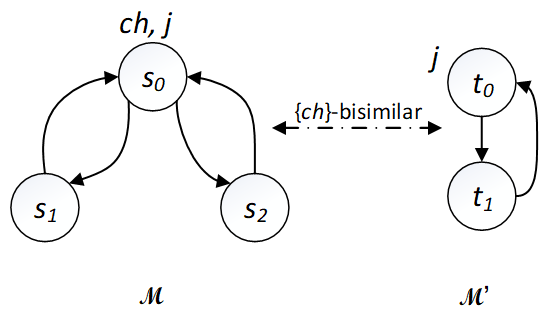
\includegraphics[width=5cm,height=3cm]{chBisimilar.png}\\
		%\vspace{2mm}
		\parbox[c]{6cm}{\footnotesize{Fig.1.~}  Two $\{ch\}$-bisimilar Kripke structures.}%\vspace*{.2mm}
	\end{center}
	
	
\end{example}

Moreover, we can see that the relation $\lrto_V$ has some interesting properties in addition to the equivalence relation. Formally:

\begin{proposition} \label{pro:EqUnion}
	Let $V, V_1 \subseteq \Ha$ and $\Hm_1$, $\Hm_2$ and $\Hm_3$ be three Kripke structures, then we have:
	\begin{enumerate} [(i)]
		\item $\lrto_V$ is an equivalence relation between Kripke structures;
		\item if $\Hm_1 \lrto_V \Hm_2$ and $\Hm_2 \lrto_{V_1} \Hm_3$, then $\Hm_1 \lrto_{V \cup V_1} \Hm_3$.
	\end{enumerate}
	
\end{proposition}

Intuitively, property (i) in Proposition~\ref{pro:EqUnion} means that $\lrto_V$ is reflexive, symmetric, and transitive.
(ii) indicates that if a Kripke structure is $V$ and $V_1$-bisimilar to the other two Kripke structures respectively, then those two Kripke structures are $V \cup V_1$-bisimilar.
As we will show in the following context, it is important to demonstrate the \emph{modularity}, one of the important properties of forgetting in $\mu$-calculus.

%Moreover, as was stated in~\cite{d1996uniform} that any ${\cal L}$-sentence $\varphi$ (that is, a $\mu$-sentence
%that uses only symbols from the language ${\cal L}$) is invariant for ${\cal L}$-bisimulation,  i.e., if there is an ${\cal L}$-bisimulation between $\Hm$ and $\Hm'$, then $\varphi$ holds in $\Hm$ iff it holds in $\Hm'$.
%In this case, it should then be apparent that if $\IR(\varphi, V)$ and
%$\Hm \lrto_V \Hm'$, then $\varphi$ holds in $\Hm$ iff it holds in $\Hm'$.
%In this paper, we call this property \emph{$V$-invariant}.


We now define forgetting in $\mu$-calculus.

\begin{definition}[Forgetting]\label{def:V:forgetting}
	Let $V\subseteq\cal A$ and $\phi$ be a $\mu$-sentence.
	A $\mu$-sentence $\psi$ with $\Var(\psi)\cap V=\emptyset$
	is a {\em result of forgetting $V$ from} $\phi$ if
	\begin{equation*}
		\Mod(\psi)=\{\Hm  \mid \exists \Hm' \in\Mod(\phi)\ \&\ \Hm' \lrto_V \Hm\}.
	\end{equation*}
\end{definition}

%For convenience, we denote the result of forgetting $V$ from $\phi$ as $\Muforget(\phi, V)$.
We denote the result of forgetting $V$ from $\phi$ as $\Muforget(\phi, V)$.
It is not difficult to see that Definition~\ref{def:V:forgetting} implies that if both $\psi$ and $\psi'$ are results of forgetting $V$ from $\phi$, then
$\Mod(\psi)=\Mod(\psi')$, i.e., $\psi$ and $\psi'$ have the same models. In this sense, the result of  forgetting $V$ from $\phi$ is unique up to semantic equivalence.

It is worthy of note that D'Agostino at al. studied the notion of \emph{uniform interpolation} in $\mu$-calculus, and inicated that $\mu$-calculus has the uniform interpolation property~\cite{d1996uniform,d2006modal}. Informally, this means that for every $\mu$-sentence $\varphi$ and every finite set $V\subseteq \Var(\varphi)$, there exists a $\mu$-sentenc $\widetilde{\exists}V \varphi$ which does not contain atoms from $V$ but is logically closest to $\varphi$ in some sense.

We should mention that our forgetting definition $\Muforget(\phi, V)$ is equivalent to the semantic definition of formula in~\cite{d2006modal}.

\clearpage
\bibliographystyle{splncs04}
\bibliography{muRef}






\clearpage
\appendix
\section{Supplementary Material: Proof Appendix}













\end{document}
